\chapter{Implementation}
The objective of this part of the project was to implement an immersive replication of \acp{ASC} induced by classical psychedelics. In order to achieve a high degree of immersion, our solution was designed to be intended for immersive \ac{VR} systems with \acp{HMD}. Our solution will be referred to with \textit{``the application''} or \textit{``our application''} for the rest of this document.

To represent the \acp{ASC} of classical psychedelics objectively, we had to resort to modelling only the ``perceptual level'' stage of the psychedelic experience (as seen in \ref{fig:temporal-dynamics}), as further stages require subjective personalization of content, and aspects less suitable for replication via immersive \ac{VR}, such as cognitive effects and the suppression of the \textit{phenomenological ego}.

\section{Design of the Application}
The application was designed primarily for the evaluation of the implemented replication. The development of the application consisted of 3 distinct parts:

\begin{enumerate}
    \item \textbf{The environment}: A virtual scene that should look as realistic as possible.
    \item \textbf{The replication}: Implementation of the effects themselves.
    \item \textbf{Adaptation for testing}: Getting the application ready for a study, that might measure the impact of the replication on the human mind.
\end{enumerate}

\subsection{Safety}
In order to ensure our application's users safety, we have consulted the \textit{Recommendations for good scientific practice and the consumers of VR-technology} \autocite{madary2016real}. The application was developed according to these recommendations.

Mainly, we don't expect the developed application to have lasting traumatic effects on the users; instead, we believe that this medium may be a suitable way to explore aspects of psychedelic-induced \acp{ASC} while minimizing those risks.

Further, we've taken safety and intuitiveness into account while designing the controls and choosing a suitable testing area for experimentation with \ac{VR} (the ``\ac{VR} play space'').

Finally, the application must be automated, so that the administrator may assist the user and ensure their safety during the usage of the application.

\subsection{Interaction}
Interaction with the scene via hand-held controllers was removed entirely, as we felt that the currently available consumer \ac{VR} technology does not implement a realistic, consistent, universal and intuitive solution for interaction with the virtual scene. For example, in \ac{VR} applications, interactions are usually implemented so that if a user takes a hand-held controller to a dynamic physics-enabled object, they may be able to pick it up by pressing or holding a trigger on the hand-held object, which makes the object stick or snap to the virtual representation of the controller in the scene. While this solution may be suitable for \ac{VR} games, it is still understood as a simplification.

As an alternative, one may consider using force feedback haptic gloves, and given a sufficient physically based simulation, it may be possible to implement realistic interactions with virtual objects. However, even such gloves apply force feedback only to the fingers and not the entire body, making it impossible to, for example, lean against virtual objects.

In any case, no such force feedback haptic gloves were available to us for this project, and so interaction was entirely foregone, in the interest of keeping the simulation focused mainly on the replication, rather than an unrealistic implementation of interactions.

\subsection{Virtual Scene Creation}
Given the goal of creating as realistic of a scene as possible, as well as no financial budget for this project, we ended up choosing \fref{https://web.archive.org/web/20220514231756/https://www.unrealengine.com/en-US}{\acf{UE4}} as the game development engine to develop our \ac{VR} application with. \ac{UE4} is free to use for projects with a lifetime gross revenue below \$1 million USD, and we have no plans to monetize it. Additionally, the choice of \ac{UE4} makes it possible to use the \fref{https://web.archive.org/web/20220514233901/https://quixel.com/megascans}{Quixel Megascans} 3D asset library for free within \ac{UE4}, due to special licensing as a result of the acquisition of Quixel by \fref{https://web.archive.org/web/20220514235540/https://www.epicgames.com/site/en-US/home}{Epic Games}, the developer of \ac{UE4}.

The virtual scene was created with the intended \textit{\ac{VR} play space} in mind, which was measured to be about $3.5\times3.5 \:\si{m^2}$ large. The virtual scene contains visual cues of the \textit{play area} borders in the form of 3D assets; specifically, the \textit{play area} is surrounded by a railing and tall rock, communicating to the user, that these objects should not be passed through.

The choice was made to create an outdoor scene, as the surrounding nature might provide a more pleasant environment than an indoor scene. However, our implementation is in no way limited to outdoor scenes only.

At first, we attempted to create a forest scene, but quickly ran into performance issues while trying to render a densely populated forest on a \ac{HMD}, which requires at least 2 views rendered at typically higher resolutions than a regular desktop screen, ideally with at least 90 \acs{FPS} (the native refresh rate of the \ac{HMD}). Delivering a consistent framerate is a requirement, as low framerates and stuttering may cause motion sickness.

It was then decided to abandon the idea of a forest scene and, instead, use a \ac{HDRI} panoramic photograph as a background (hereinafter ``panoramic background'') for the scene. It is important to note, that a panoramic background has no depth information. This drawback can be mitigated by making only the very distant parts of the panoramic background visible to the user, so that the illusion of the panoramic background being realistic is not broken. The illusion relies on the fact that binocular disparity is low for distant objects.

Close parts of the panoramic background can be hidden with 3D assets suitable for the environment. To minimize the area that needed to be hidden, we have chosen a mountainside panoramic background (see figure \ref{fig:cannon}).

\begin{figure}[H]
    \centering
    \ifgraphics
        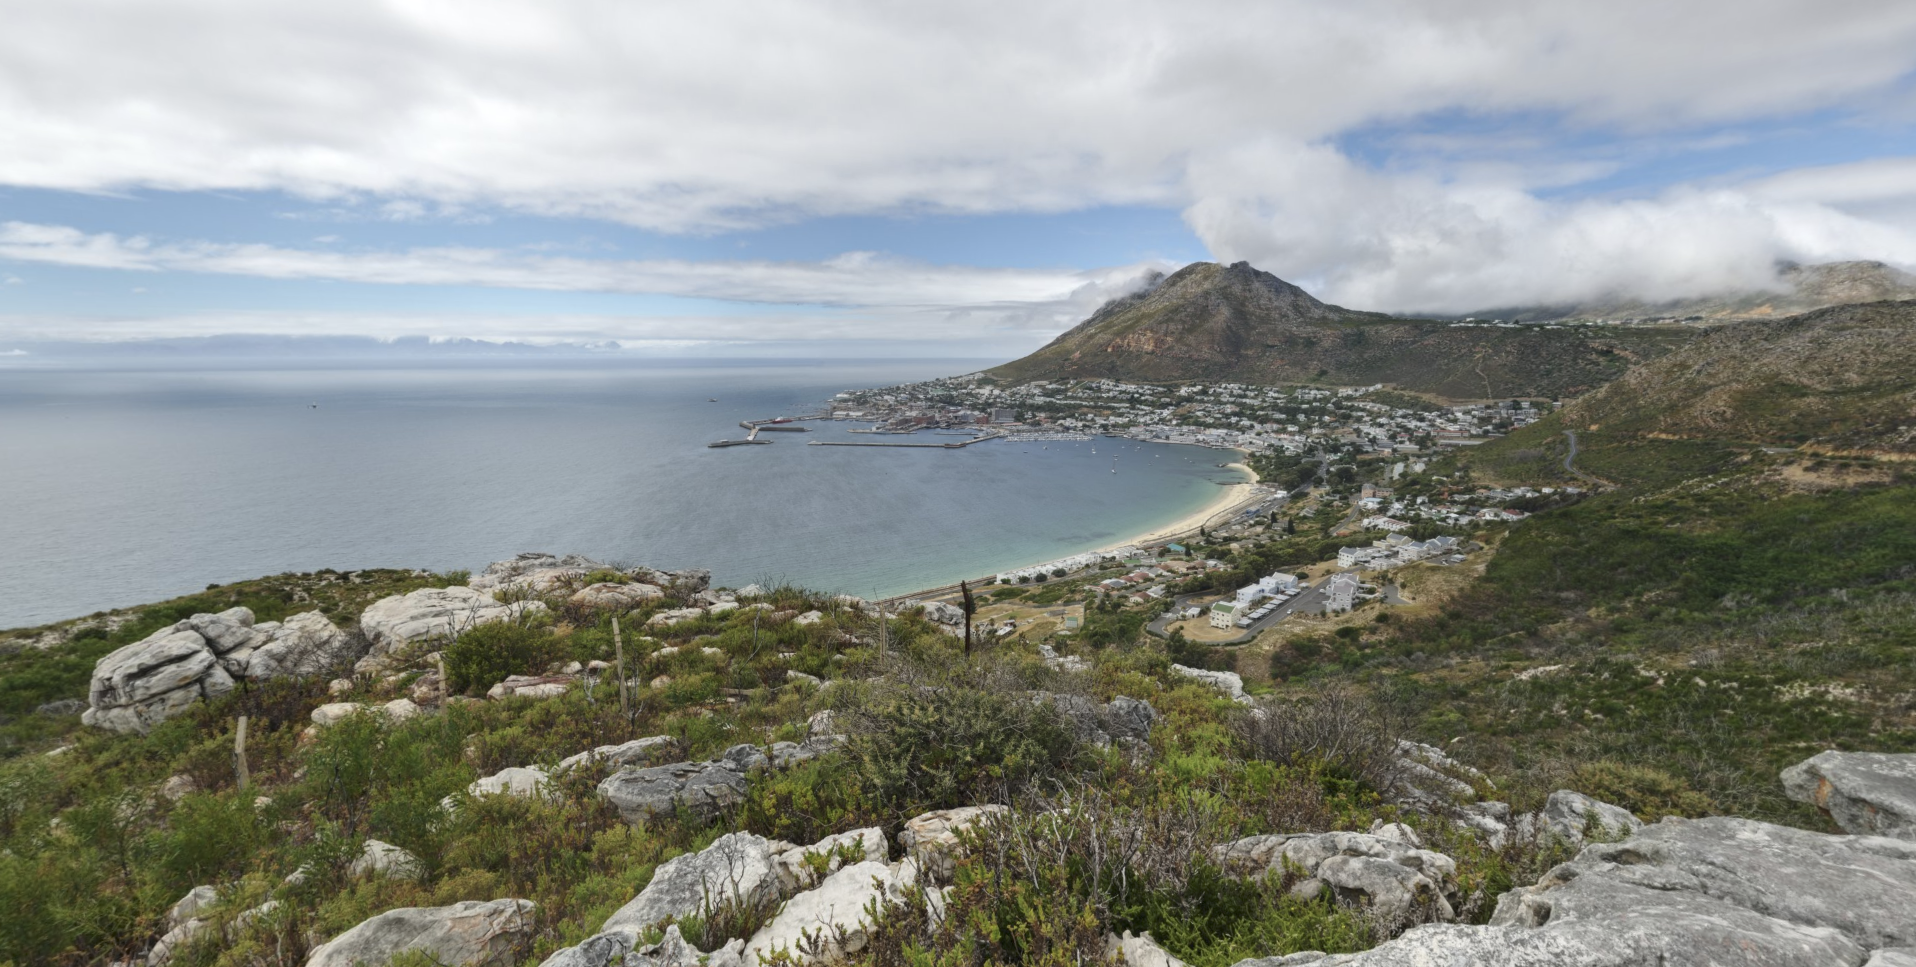
\includegraphics[width=0.95\textwidth]{img/cannon.png}
    \fi
    \caption{The chosen panoramic background ``Cannon''\cczerofootnote{Greg Zaal} available on \fref{https://web.archive.org/web/20220515010919/https://polyhaven.com/a/cannon}{Poly Haven}.}\label{fig:cannon}
\end{figure}

The final scene contains a flat patch of grass and other low foliage the size of the \textit{play area}, containing a wooden bench with some gardening tools. The grass patch is surrounded with rock formations and a rocky stairway leading towards it. Beyond the railing, there is a nice view of the sea cove.

\begin{figure}[H]
    \centering
    \ifgraphics
        TODO: image of the scene
        % 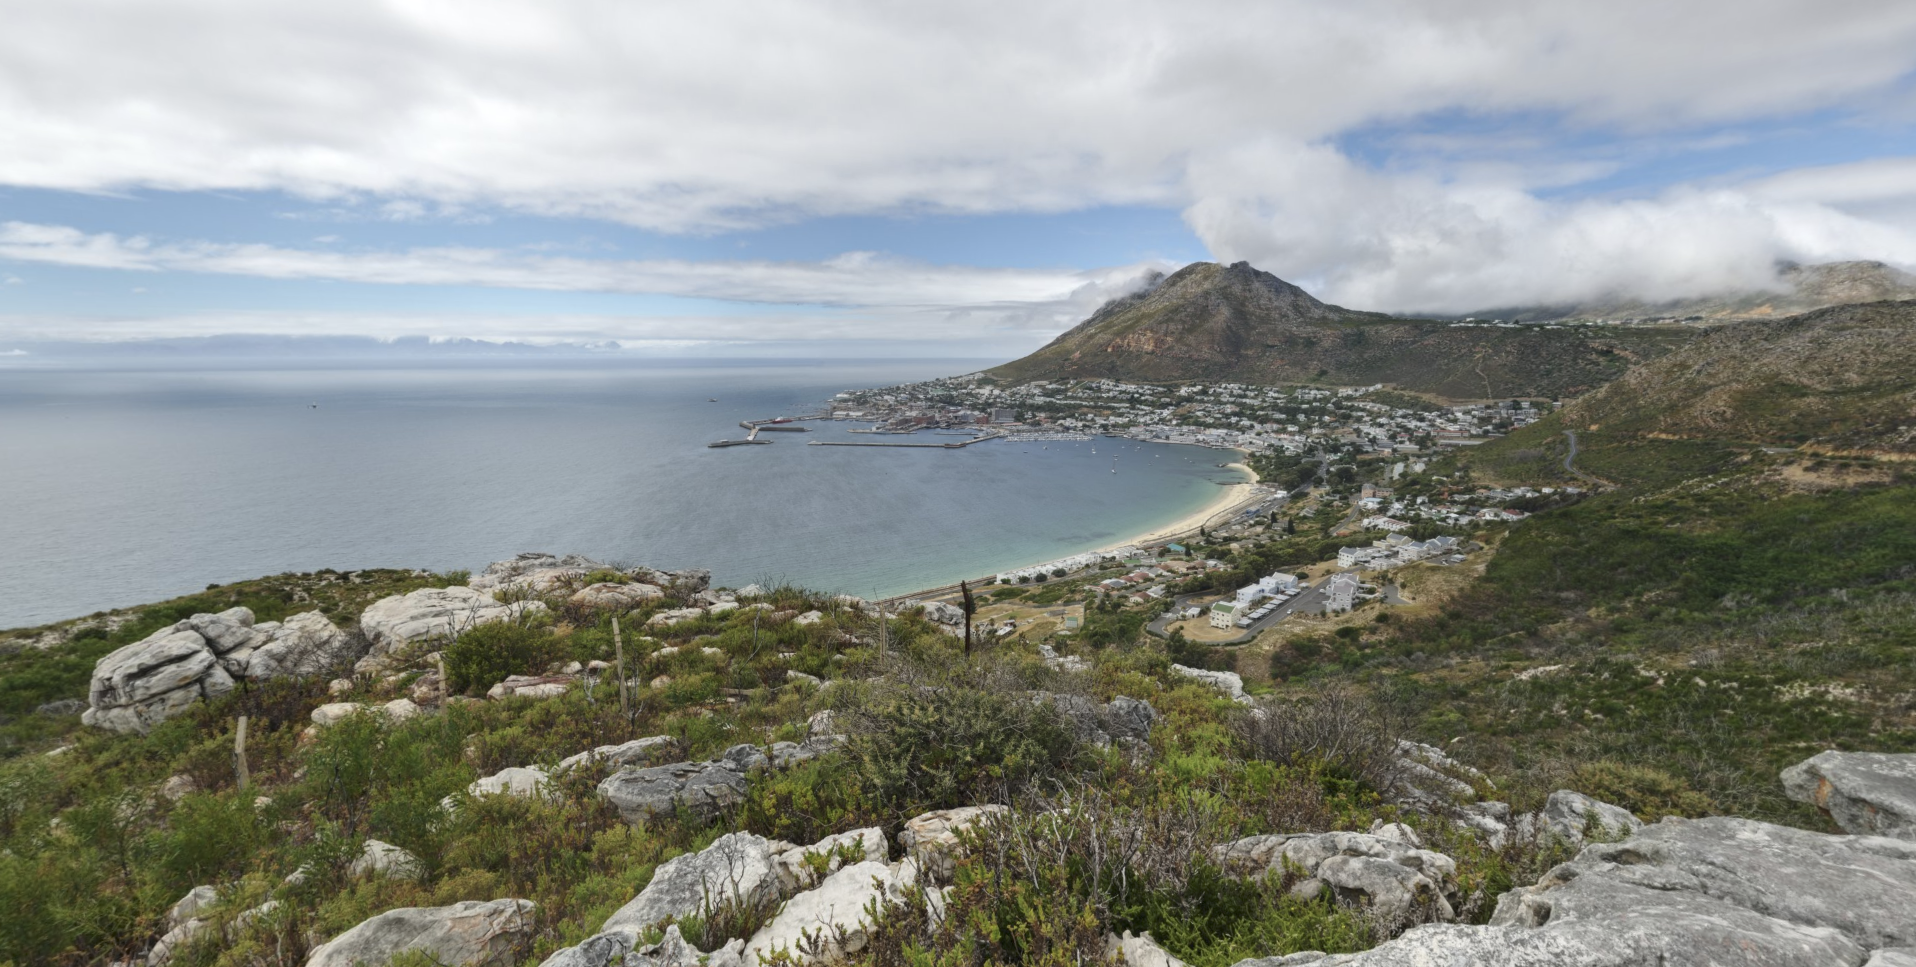
\includegraphics[width=0.95\textwidth]{img/cannon.png}
    \fi
    \caption{A preview of the resulting scene.}\label{fig:scene-preview}
\end{figure}

\section{Implementation of Replications}
\subsection{Spatial Effects}
\subsubsection{Depth Perception Distortion}

\autocite{fischer1970psilocybin}

\subsubsection{Waviness or "Breathing" of Objects}
\subsection{Non-Spatial Effects}
\subsubsection{Visual Acuity Enhancement}
\subsubsection{Hue Shifting}
\subsubsection{Tracers}
\section{Complex Replication}
\subsection{Execution Order}

\begin{figure}[H]
    \centering
    \ifgraphics
        \begin{tikzpicture}[node distance = 2cm, auto]
            \tikzstyle{block} = [rectangle, draw, fill=blue!20, text centered, rounded corners, minimum height=1em]
            \tikzstyle{line} = [draw, -latex']

            \node [block] (wiggle) {Object Waviness};
            \node [block, below=0.5cm of wiggle] (depthperception) {Depth Perception Distortion};
            \node [block, below=1.25cm of depthperception] (sharpen) {Sharpening};
            \node [block, below=0.5cm of sharpen] (tracers) {Tracers};
            \node [block, below=1.25cm of tracers] (contrast) {Contrast and Saturation};

            \node [draw, densely dotted, minimum width=12cm, inner sep=0.5cm, fit=(wiggle)(depthperception)] (scopematerial) {};
            \node [draw, densely dotted, minimum width=12cm, inner sep=0.5cm, fit=(sharpen)(tracers)] (scopeplugin) {};
            \node [draw, densely dotted, minimum width=12cm, inner sep=0.5cm, fit=(contrast)] (scopeengine) {};

            \node [below right, text width=0.5\textwidth] at (scopematerial.north west) {{\scriptsize Material Graph\\Vertex Shader}};
            \node [below right, text width=0.5\textwidth] at (scopeplugin.north west) {{\scriptsize Engine Plugin Modifying the \acs{RDG}\\Post-Processing}};
            \node [below right, text width=0.5\textwidth] at (scopeengine.north west) {{\scriptsize Engine Built-in\\Post-Processing}};

            \path [line] (wiggle) -> (depthperception);
            \path [line] (depthperception) -> (sharpen);
            \path [line] (sharpen) -> (tracers);
            \path [line] (tracers) -> (contrast);
        \end{tikzpicture}
    \fi
    \caption{The execution order of partial replications, making up the complex replication.}\label{fig:scene-preview}
\end{figure}

\subsection{Experiment Automation}\label{sec:experiment_automation}
